\section{Results and Discussion}

In DISHTINY, cellular reproduction is contingent on resource collection and cellular decision-making (e.g., to execute the ``Reproduce'' instruction) and is not directly tied to the elapsing of updates.
So, although each replicate ran for the same number of updates, the number of cellular generations elapsed differs between replicates.
Indeed, because cellular reproduction is asynchronous, extant cells within a single replicate differ with respect to number of cellular generations removed from an initial seed cell.
However, computing the mean across extant cells for cellular generations elapsed at the end of a run provides a reasonable notion of phylogenetic depth.

\begin{table}
 \centering
 \begin{tabular}{l c|cc} % alignment of each column data
 \multicolumn{4}{c}{\textbf{Elapsed Cellular Generations}} \\
 & & \multicolumn{2}{c}{Resource Wave Size} \\
 & & Small & Large \\
 \hline
 \multirow{5}{*}{\STAB{\rotatebox[origin=c]{90}{\parbox{1.5cm}{\centering Mutational\\Load}}}} & 1 & $298 \pm 234$ & $50 \pm 38$ \\
 & 2 & $224 \pm 145$ & $32 \pm 10$ \\
 & 3 & $111 \pm 22$ & $17 \pm 3$
 \\
 & 4 & $74 \pm 11$ & $11 \pm 1$ \\
 & 5 & $120 \pm 2$ & $6 \pm 1$ \\
\end{tabular}
\caption{
Number of elapsed cellular generations by treatment (mean $\pm$ standard deviation across replicates).
}
\label{tab:cell_generations}
\end{table}


Table \ref{tab:cell_generations} shows mean cellular generations elapsed at the end of an evolutionary run for each treatment.
The number of elapsed cellular generations varies systematically across treatments, generally deceasing both with increasing mutational load and increased resource wave size.
Across treatments, elapsed cellular generation counts range from around 298 to around 6.

Large resource wave size may depress the cellular generation rate for two reasons.
Because of their reduced radius and duration, in our implementation small resource wave events occur more densely and more frequently.
Although each small resource wave dispenses less resource compared to large resource wave, the small resource wave replicates enjoy greater average resource availability per update.
In addition, forming the small same-channel groups required to fully exploit small resource waves is a less challenging task than forming the large same-channel groups required to fully exploit large resource waves.

There are also two reasons why mutational load may depress the cellular generation rate.
First, because mutations cause some proportion of reproduction events to result in dead offspring (e.g., offspring that execute an ``Apoptosis'' instruction) or sterile offspring (e.g., offspring that fail to execute the ``Reproduce'' instruction ), higher mutational load may inherently depress the growth rate of the population.
Second, higher mutational load may make developing and maintaining cooperative same-channel resource collection groups more difficult, therefore suppressing the resource collection rate.
For example, under greater mutational load same-channel resource collection groups may have to contend with members that unnecessarily expend resource replacing existing members with their offspring instead of growing the group, disrupt the group by inserting offspring with a new channel ID at the interior of the group, or hog resource that may otherwise be shared between group members.

\begin{figure}[!htbp]
\begin{center}
\rotatebox{90}{~~~~~Mutational Load 1}
\begin{subfigure}[b]{0.45\columnwidth}
  \centering
  Small Resource Wave\\~\\
  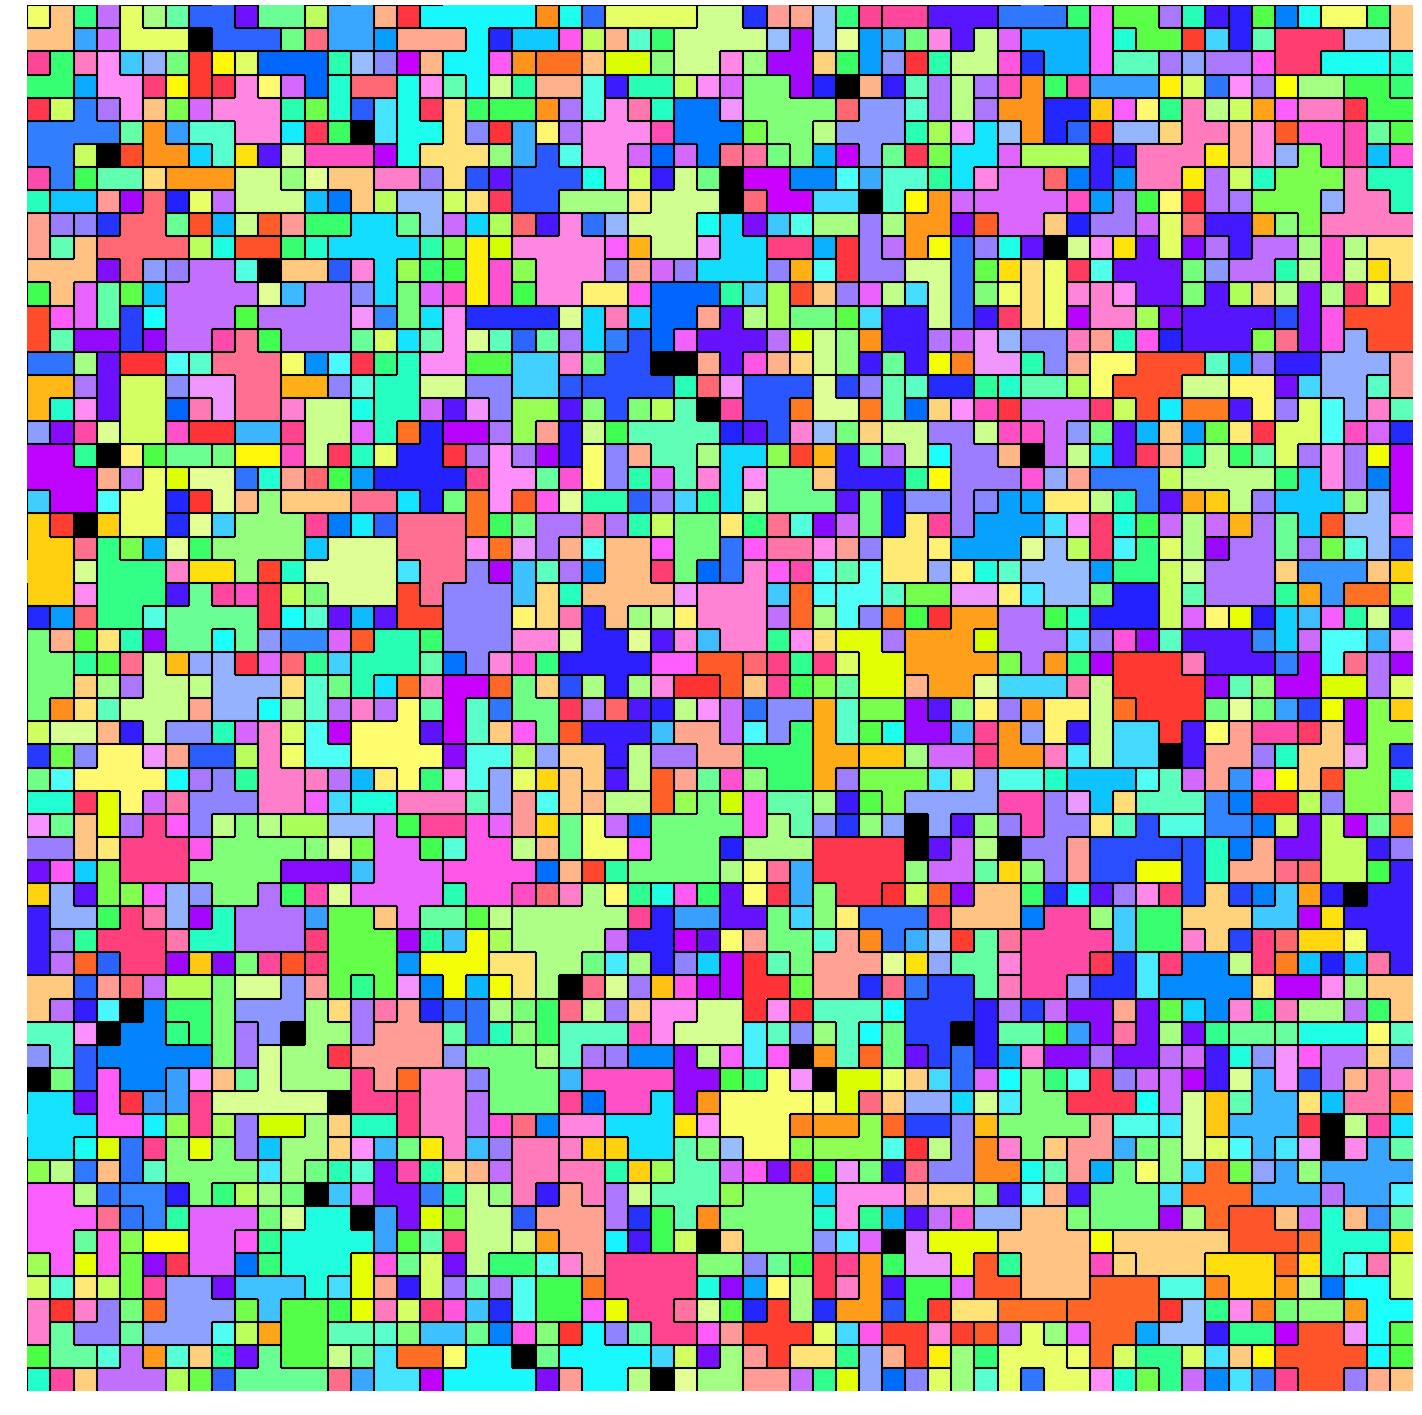
\includegraphics[width=\columnwidth]{seed=1001+title=channel_viz+treat=wave-small__mut-a_low+update=50000+_data_hathash_hash=38f284fb779ed3f5+_script_fullcat_hash=474b4115ecde8750+_source_hash=d53f428-clean+ext=}
\end{subfigure}
\begin{subfigure}[b]{0.45\columnwidth}
  \centering
  Large Resource Wave\\~\\
  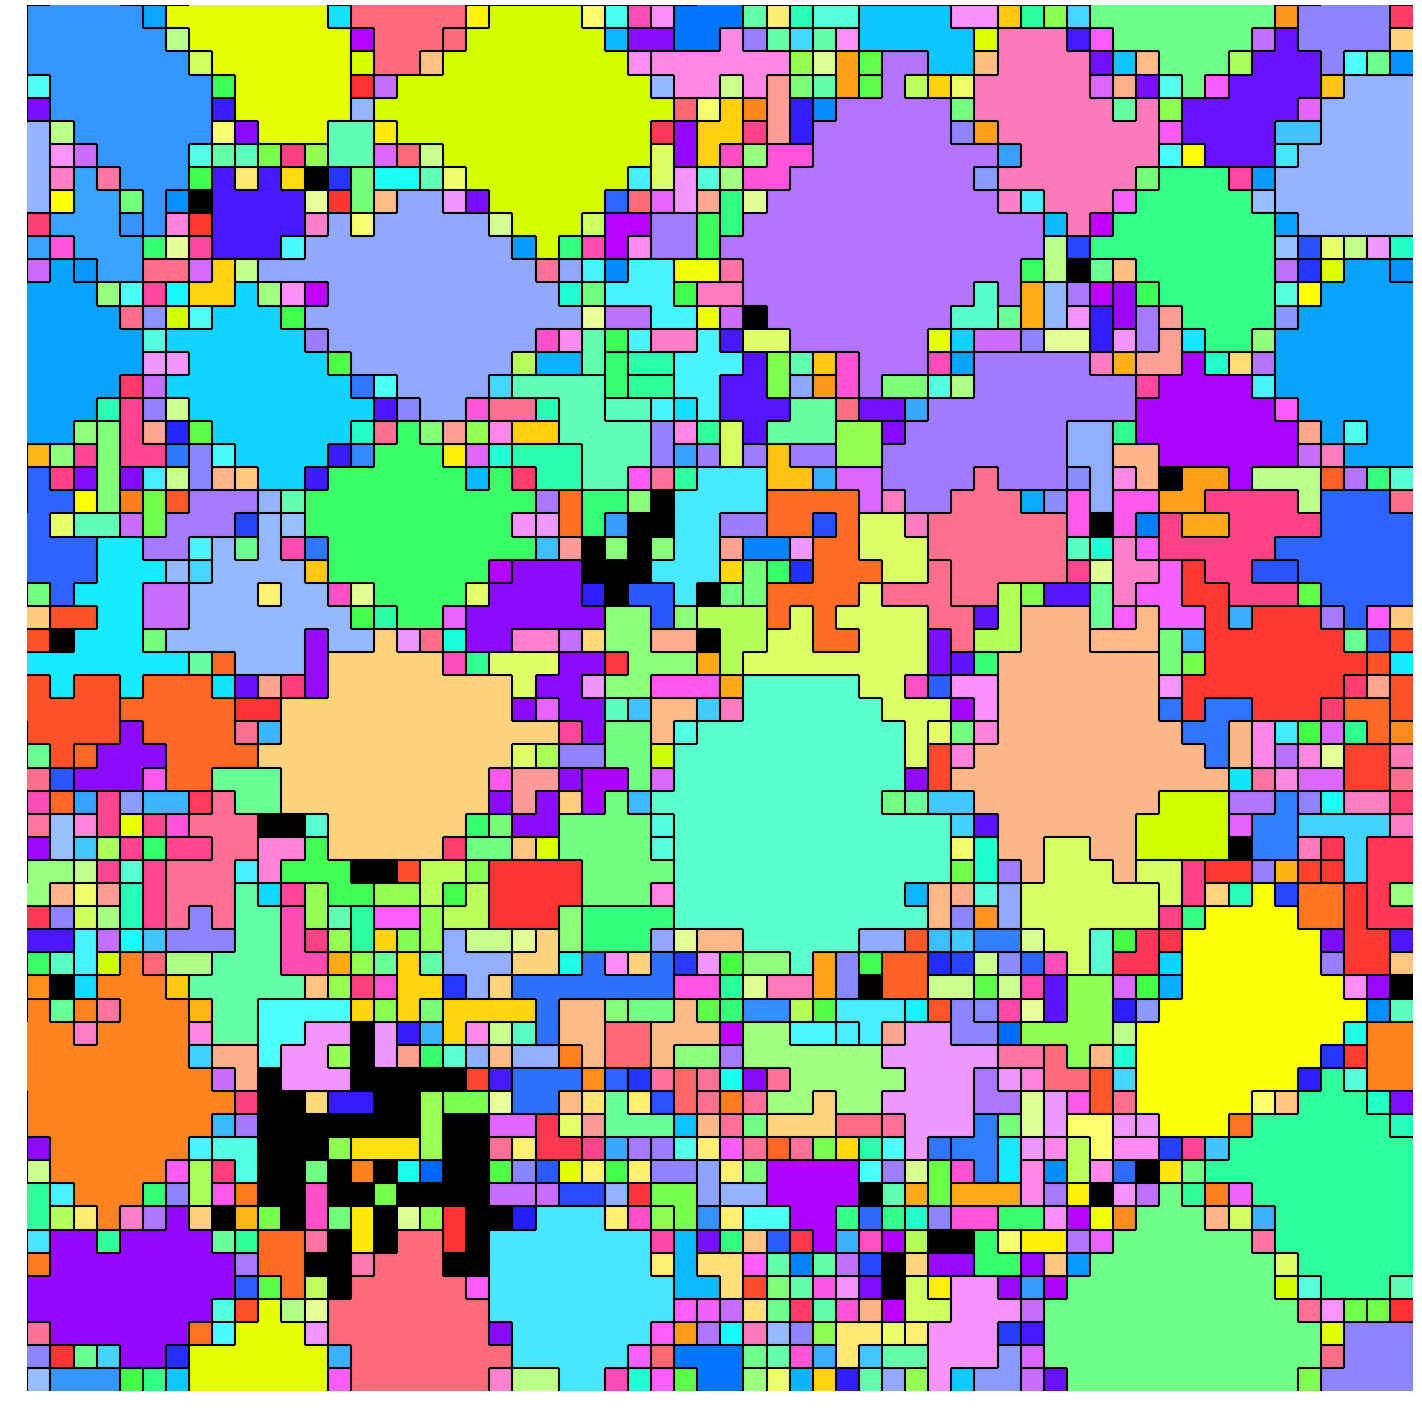
\includegraphics[width=\columnwidth]{seed=1001+title=channel_viz+treat=wave-big__mut-a_low+update=50000+_data_hathash_hash=33ac6f19e90e7ab9+_script_fullcat_hash=474b4115ecde8750+_source_hash=d53f428-clean+ext=}
\end{subfigure}

\rotatebox{90}{~~~~~~~Mutational Load 2}
\begin{subfigure}[b]{0.45\columnwidth}
  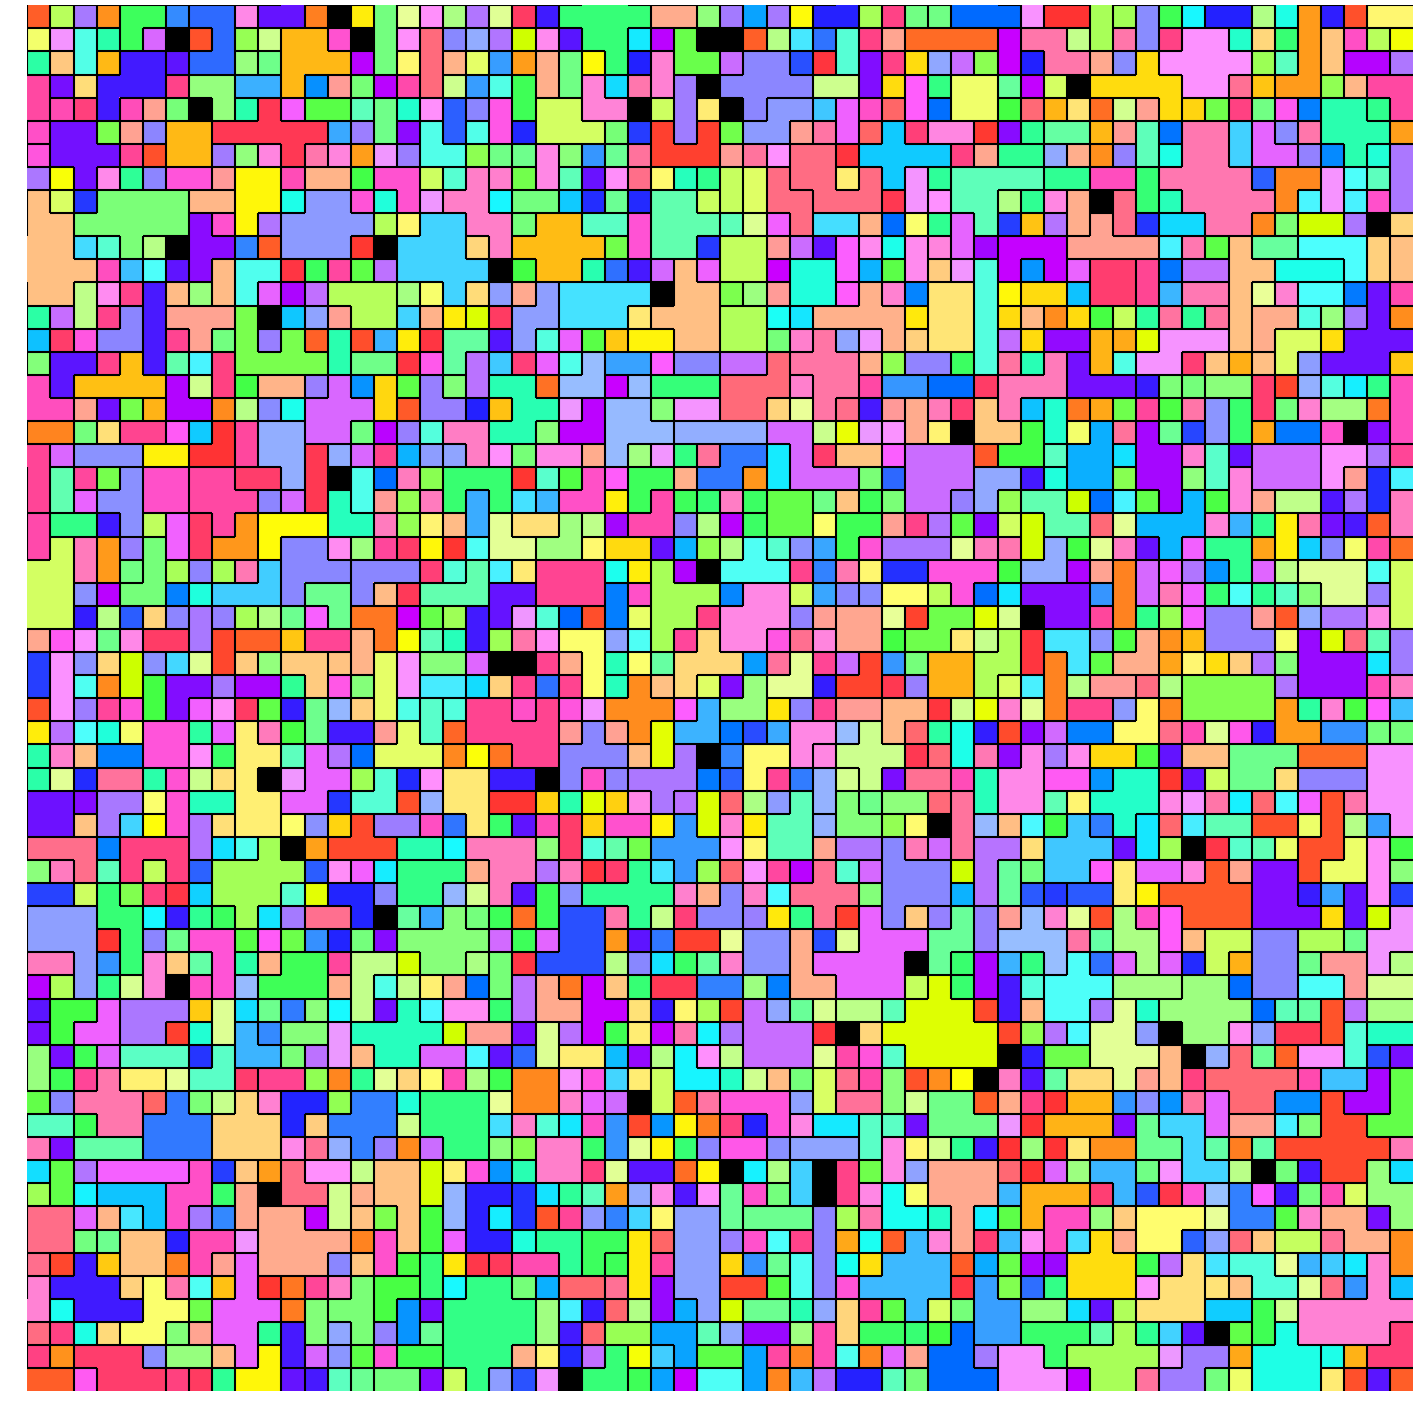
\includegraphics[width=\columnwidth]{seed=1001+title=channel_viz+treat=wave-small__mut-b_medlow+update=50000+_data_hathash_hash=0c0190afbbcd9acb+_script_fullcat_hash=474b4115ecde8750+_source_hash=d53f428-clean+ext=}
\end{subfigure}
\begin{subfigure}[b]{0.45\columnwidth}
  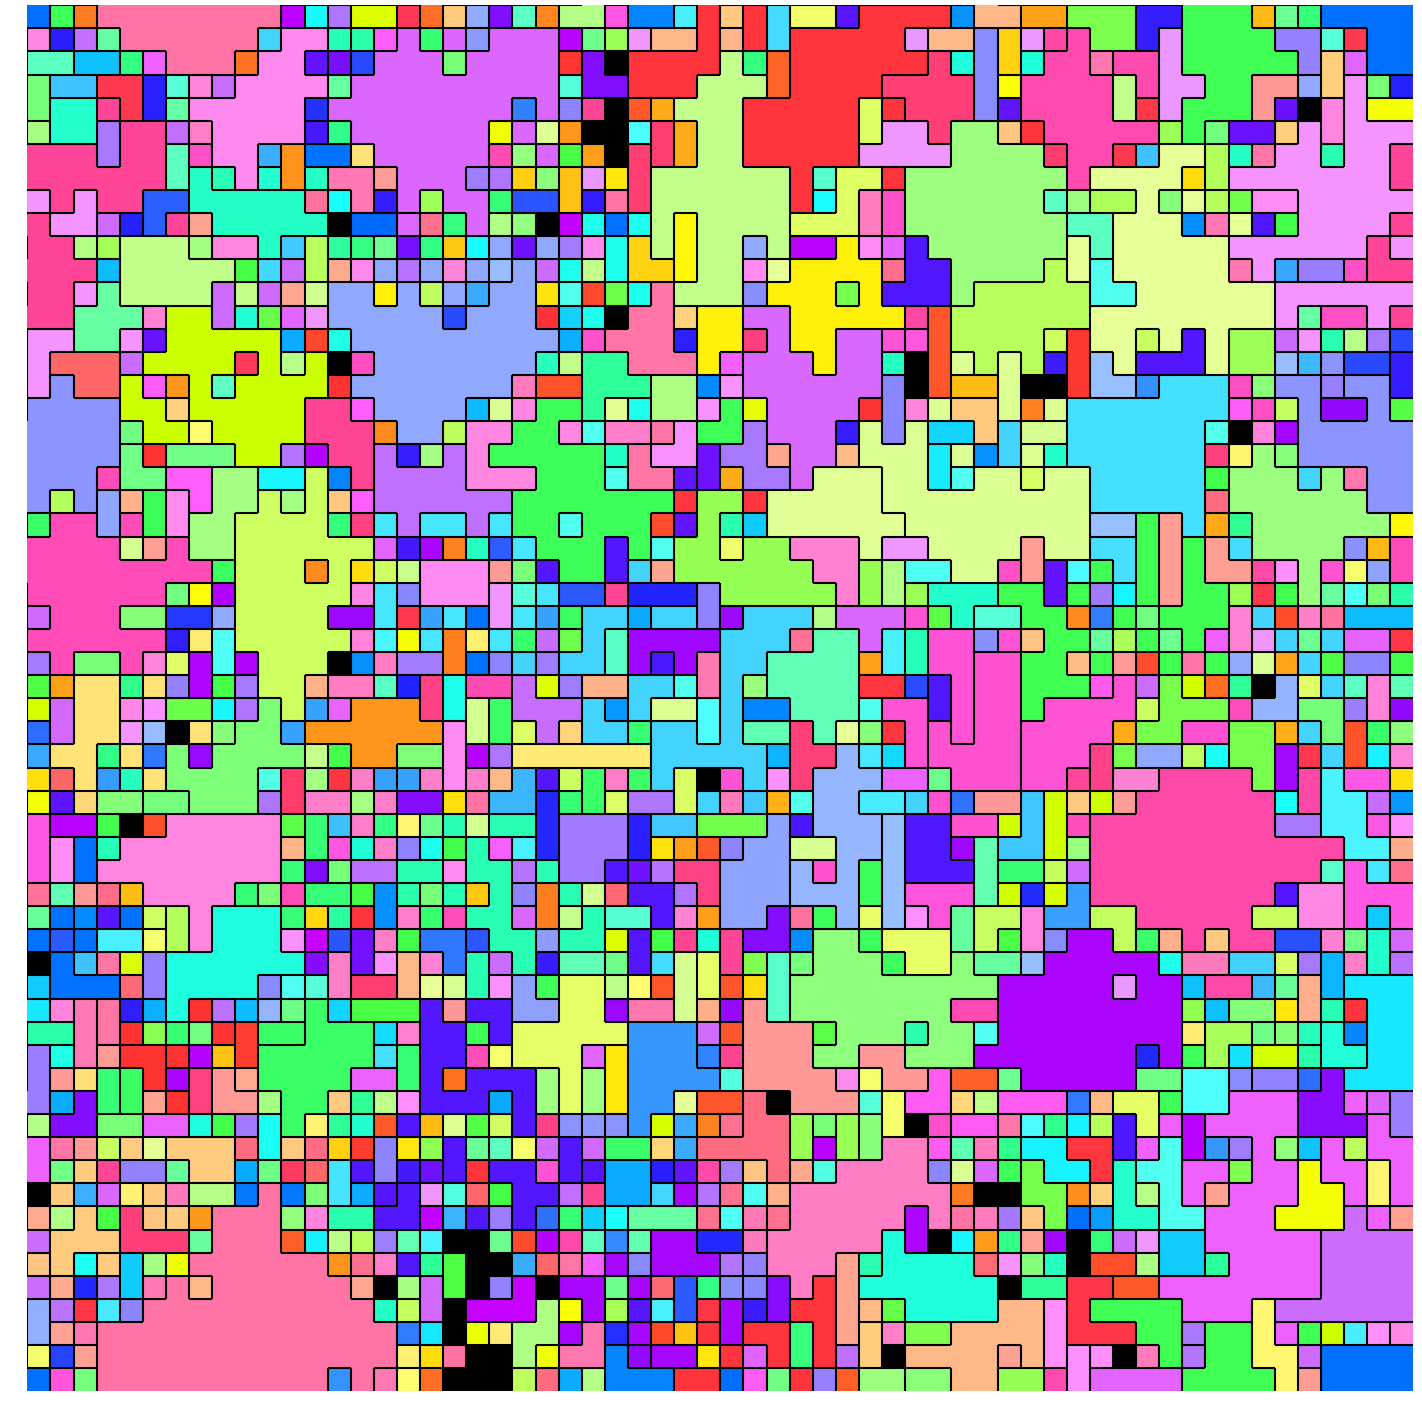
\includegraphics[width=\columnwidth]{seed=1001+title=channel_viz+treat=wave-big__mut-b_medlow+update=50000+_data_hathash_hash=50427fb0ffaf976a+_script_fullcat_hash=474b4115ecde8750+_source_hash=d53f428-clean+ext=}
\end{subfigure}

\rotatebox{90}{~~~~~~~Mutational Load 3}
\begin{subfigure}[b]{0.45\columnwidth}
  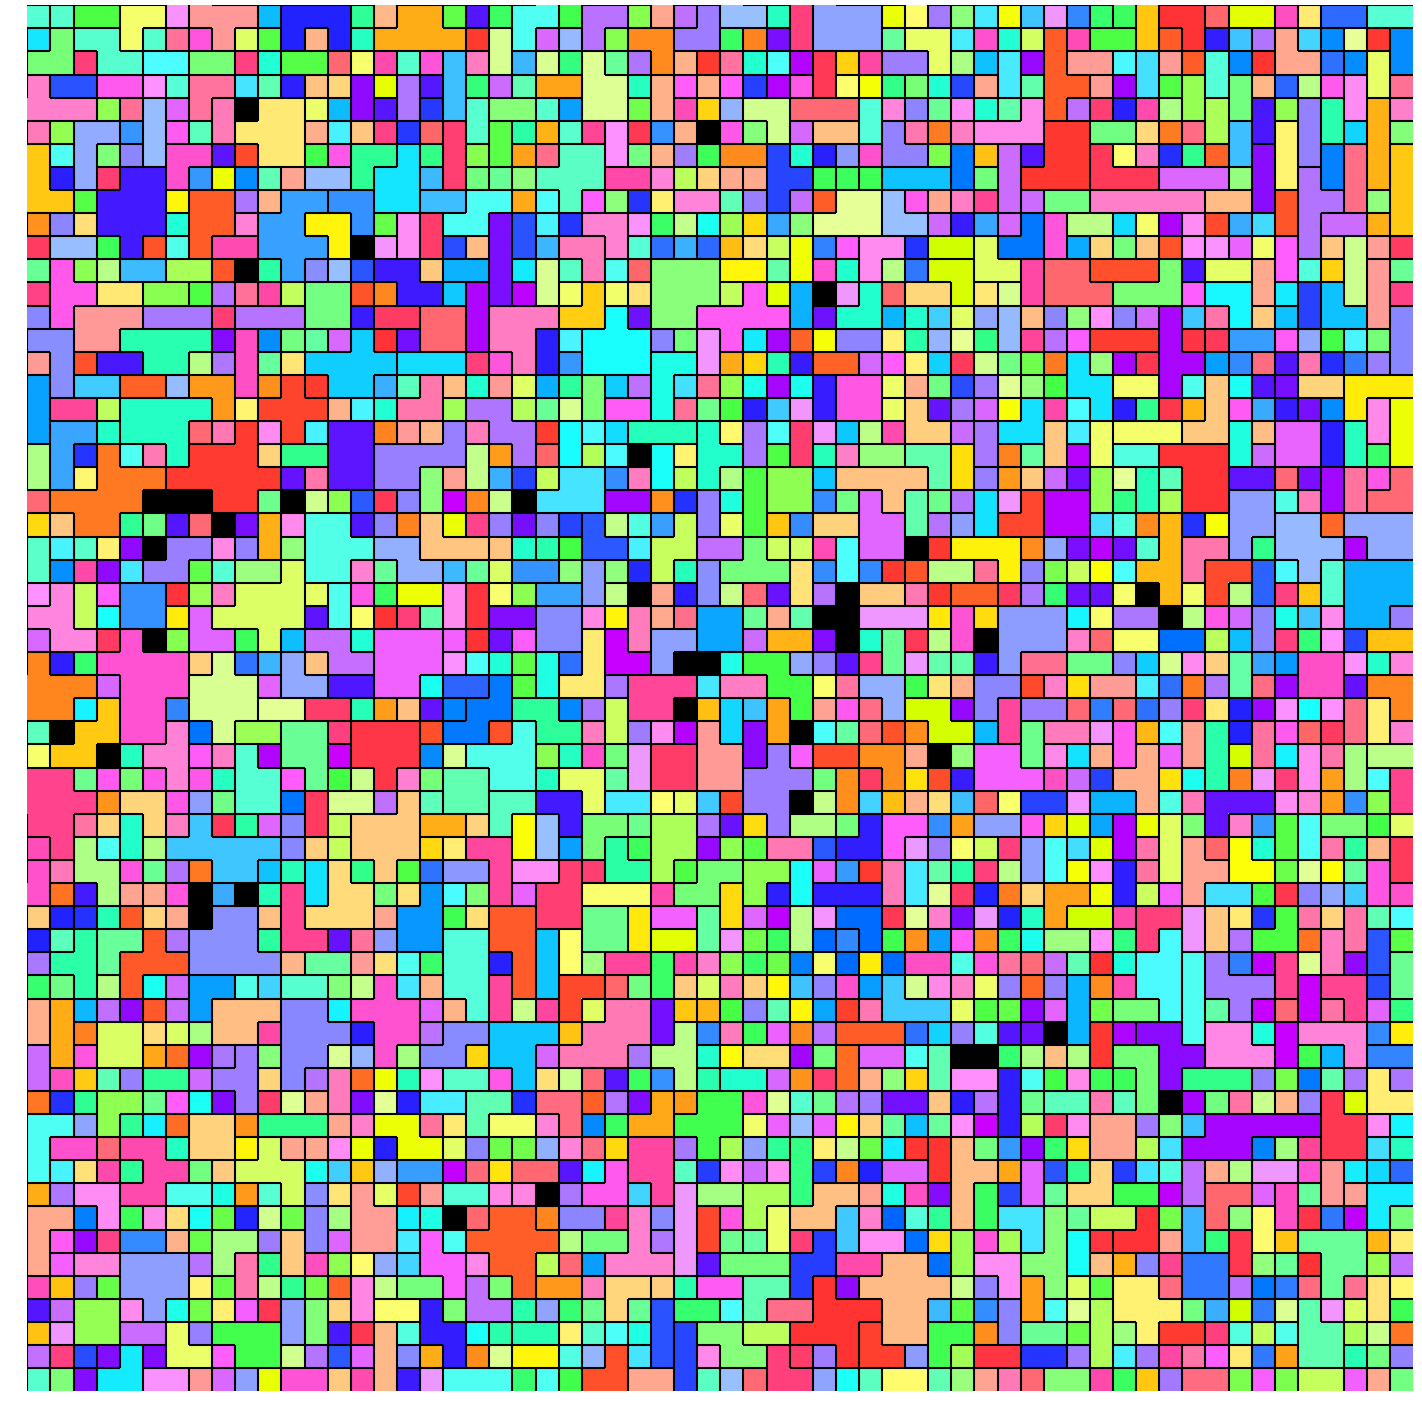
\includegraphics[width=\columnwidth]{seed=1001+title=channel_viz+treat=wave-small__mut-c_medhigh+update=50000+_data_hathash_hash=153e2f8791347e2b+_script_fullcat_hash=474b4115ecde8750+_source_hash=d53f428-clean+ext=}
\end{subfigure}
\begin{subfigure}[b]{0.45\columnwidth}
  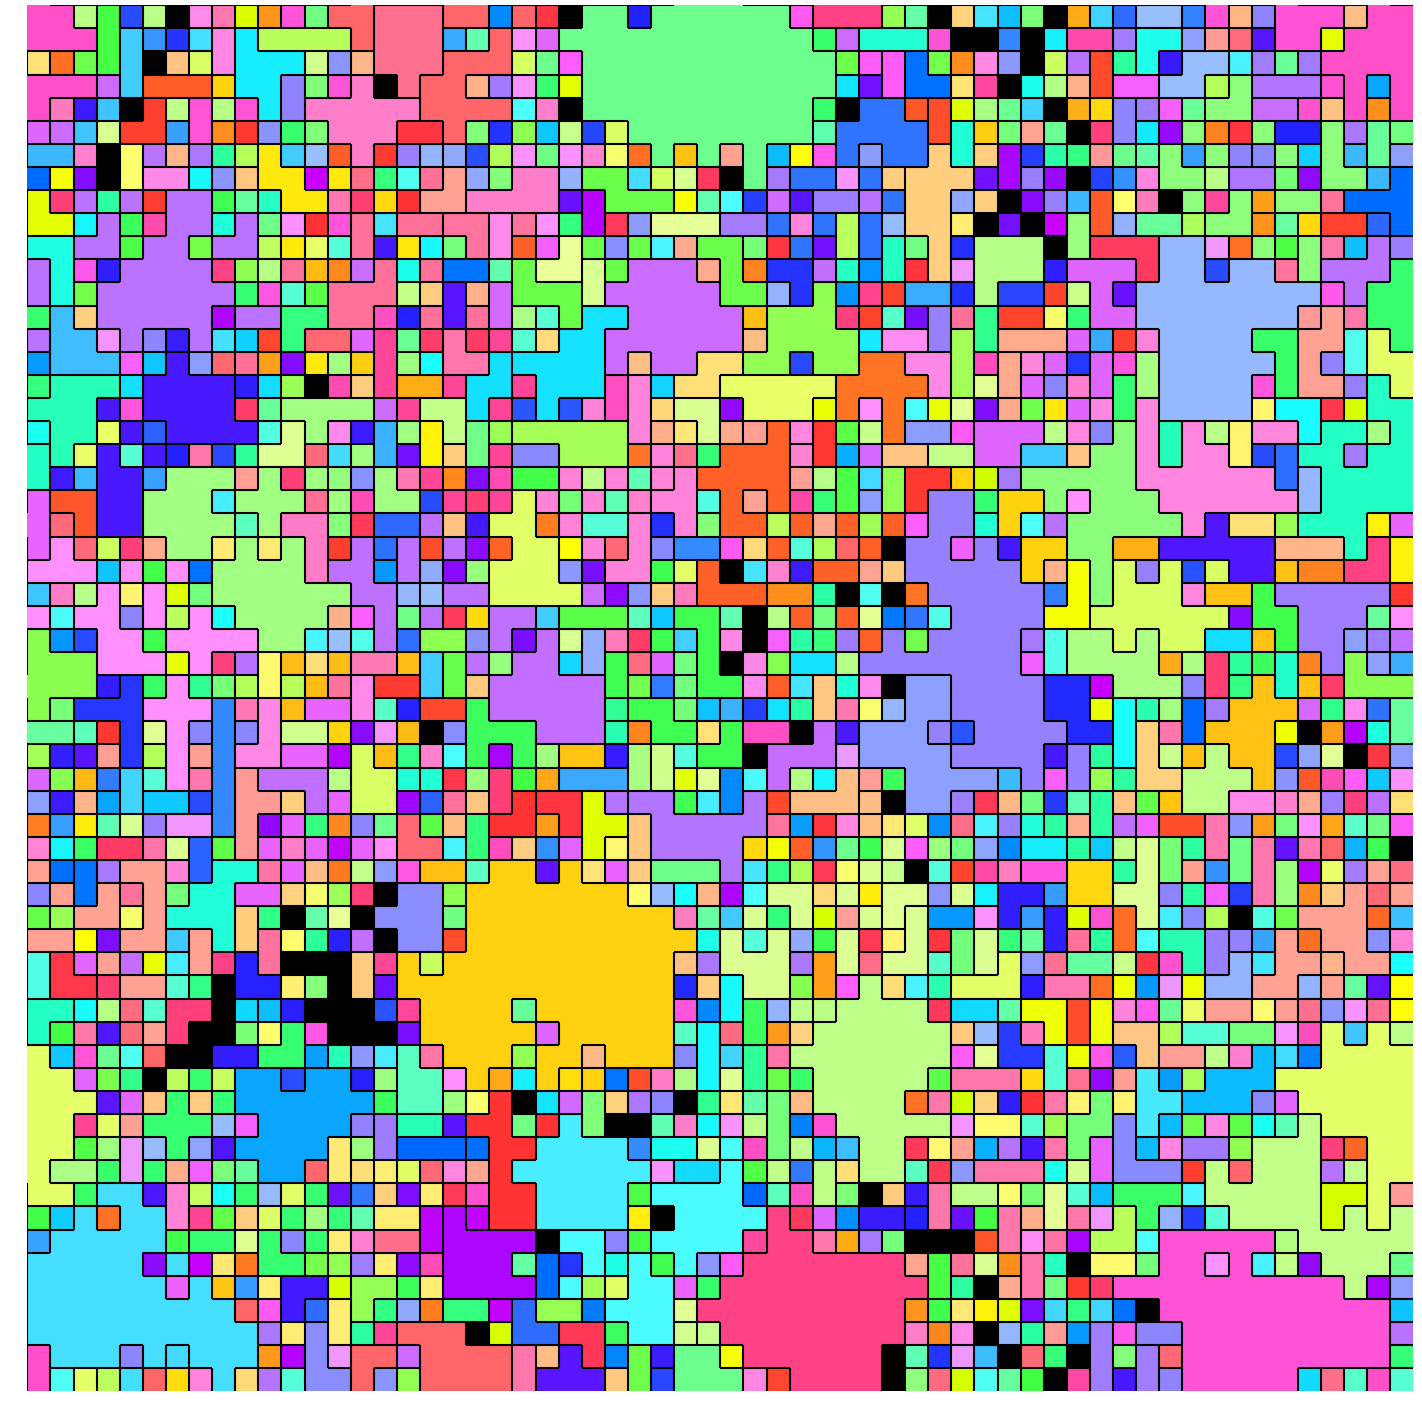
\includegraphics[width=\columnwidth]{seed=1001+title=channel_viz+treat=wave-big__mut-c_medhigh+update=50000+_data_hathash_hash=3bc8464cdb13317c+_script_fullcat_hash=474b4115ecde8750+_source_hash=d53f428-clean+ext=}
\end{subfigure}

\rotatebox{90}{~~~~~~~Mutational Load 4}
\begin{subfigure}[b]{0.45\columnwidth}
  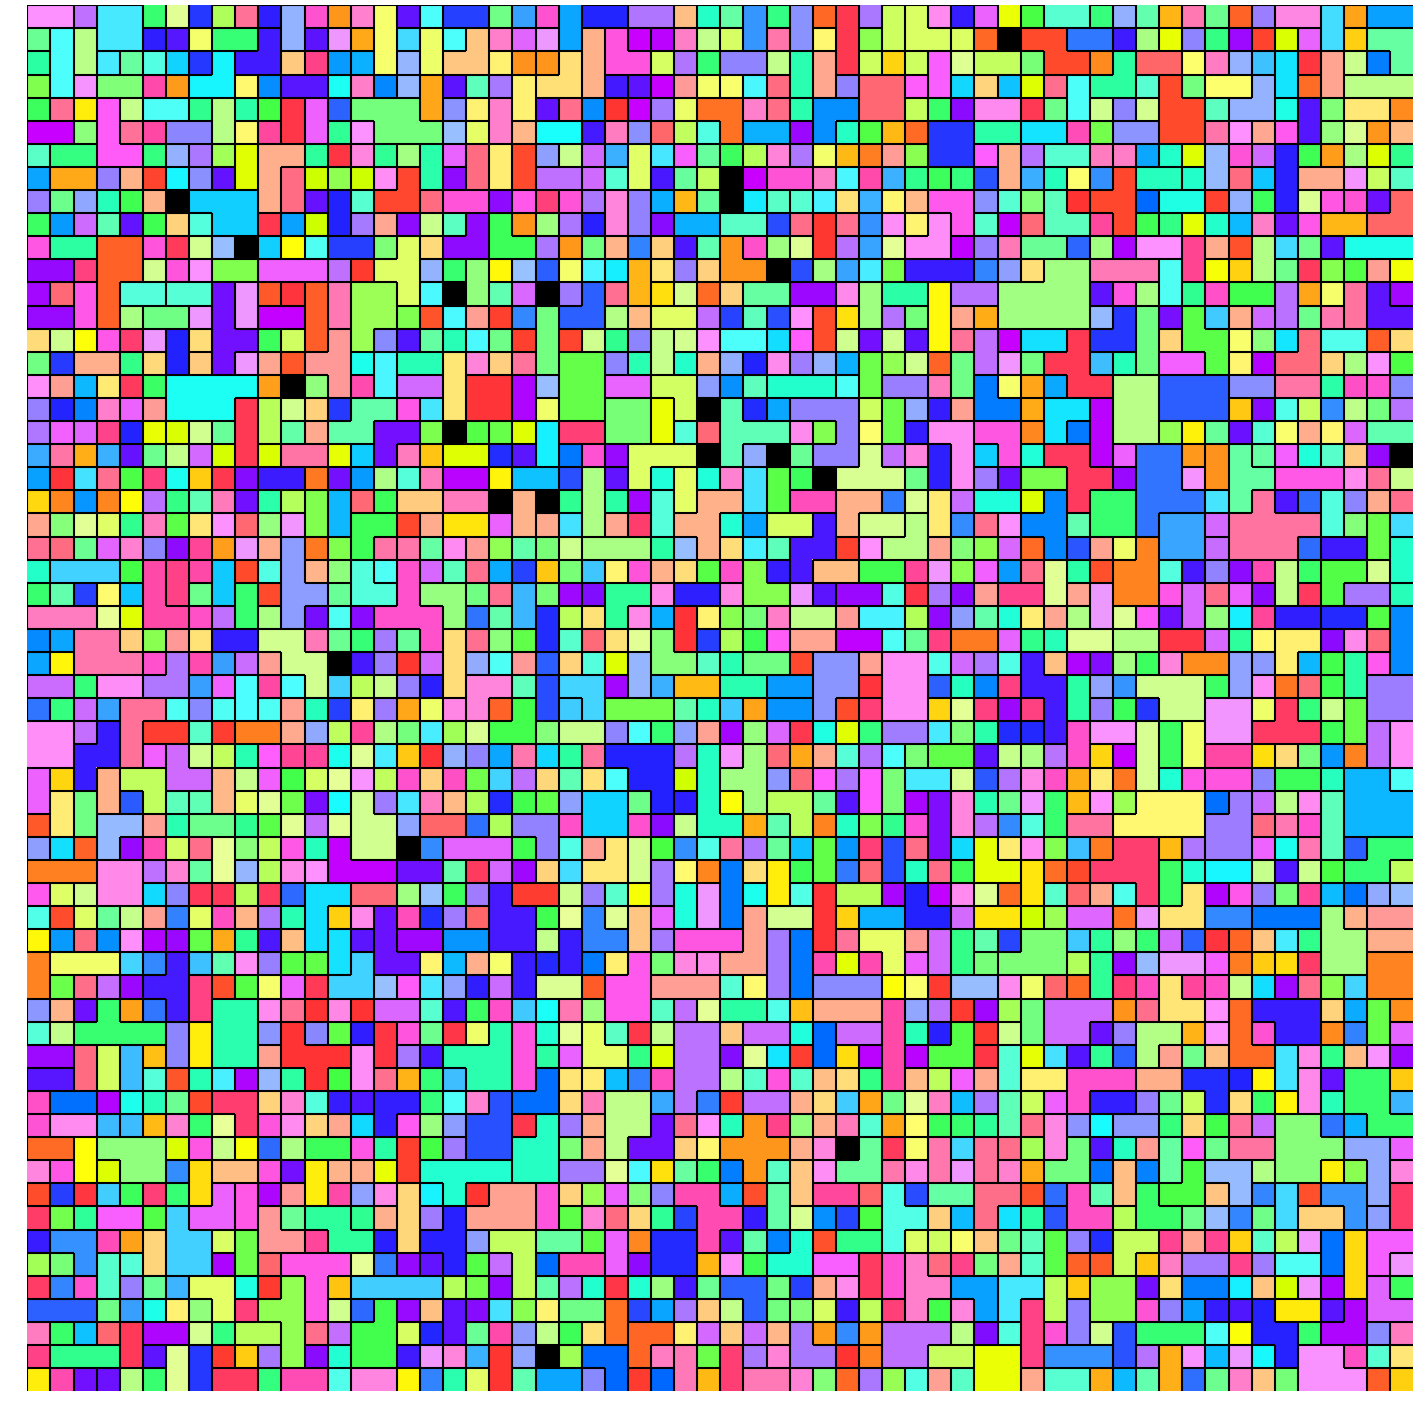
\includegraphics[width=\columnwidth]{seed=1001+title=channel_viz+treat=wave-small__mut-d_high+update=50000+_data_hathash_hash=700947e5ae80d046+_script_fullcat_hash=474b4115ecde8750+_source_hash=d53f428-clean+ext=}
\end{subfigure}
\begin{subfigure}[b]{0.45\columnwidth}
  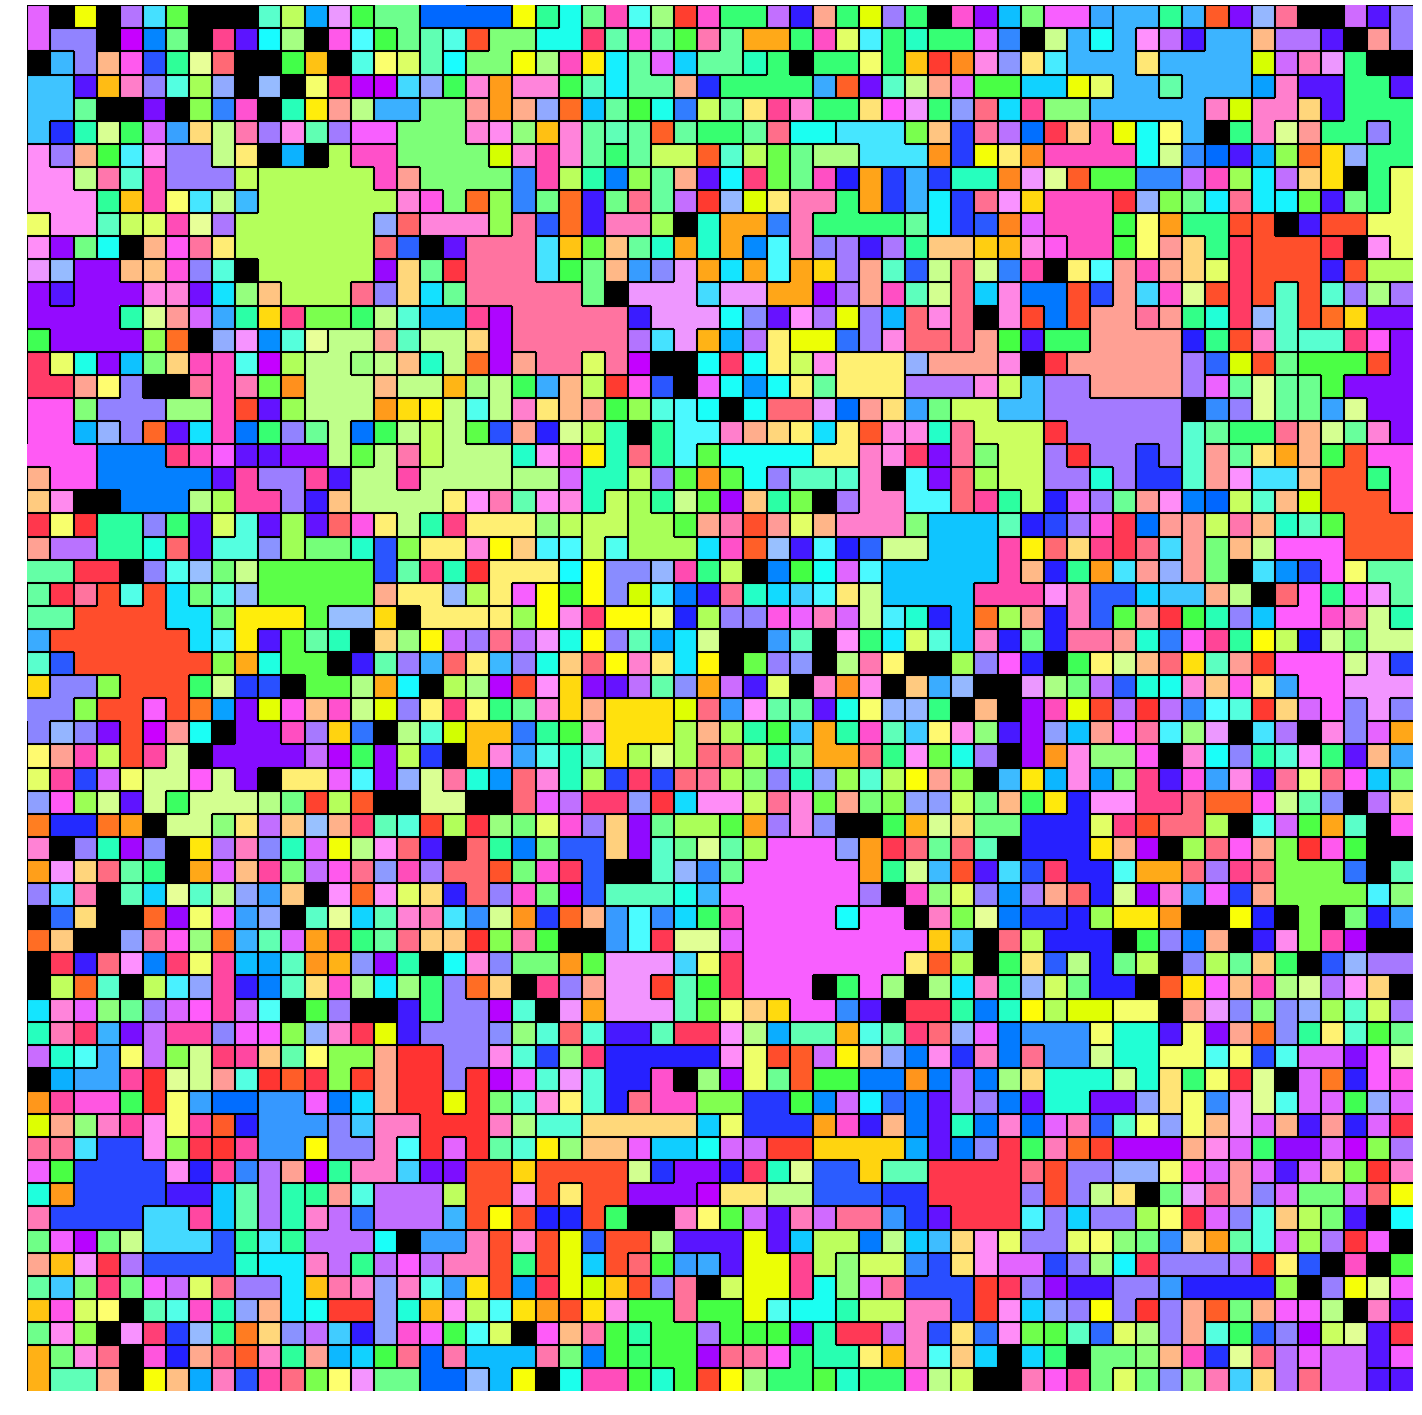
\includegraphics[width=\columnwidth]{seed=1001+title=channel_viz+treat=wave-big__mut-d_high+update=50000+_data_hathash_hash=e7071e390f076a00+_script_fullcat_hash=474b4115ecde8750+_source_hash=d53f428-clean+ext=}
\end{subfigure}

\rotatebox{90}{~~~~~~~Mutational Load 5}
\begin{subfigure}[b]{0.45\columnwidth}
  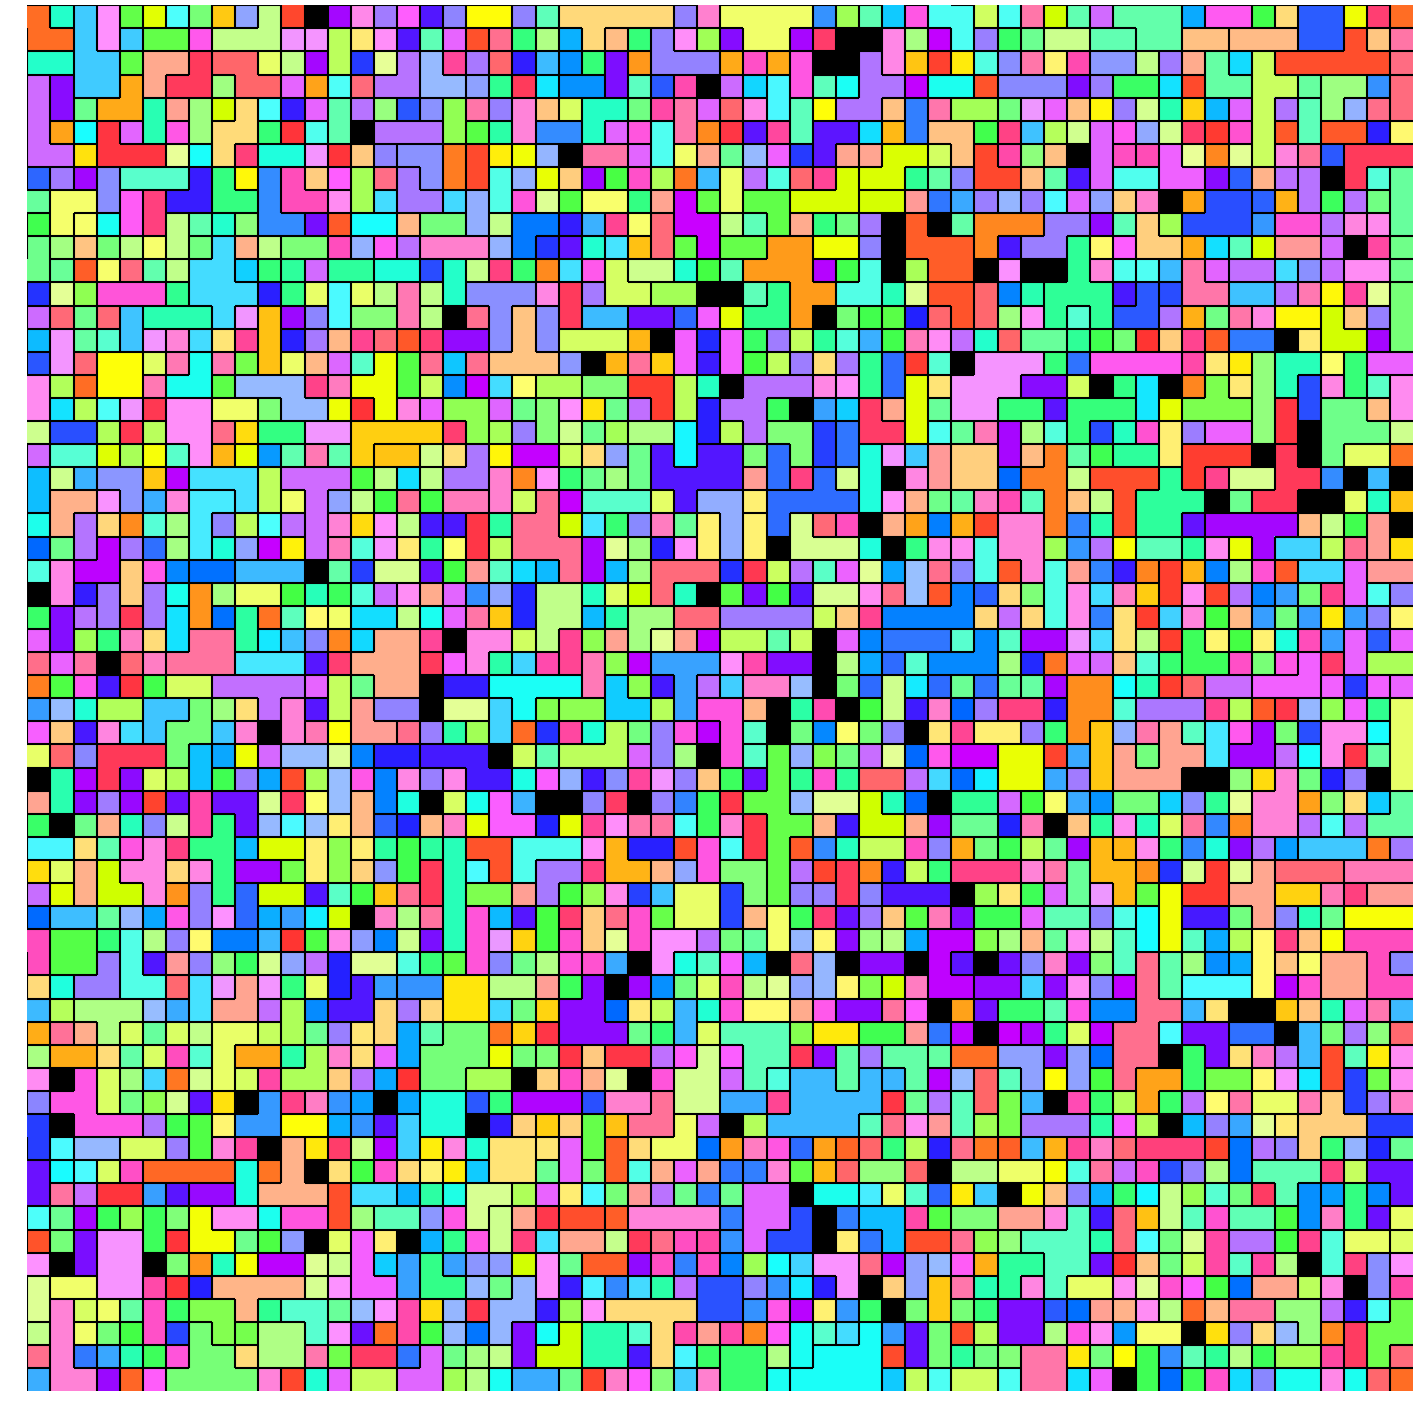
\includegraphics[width=\columnwidth]{seed=1001+title=channel_viz+treat=wave-small__mut-e_extreme+update=50000+_data_hathash_hash=70d59bcccb7f3ca6+_script_fullcat_hash=474b4115ecde8750+_source_hash=d53f428-clean+ext=}
\end{subfigure}
\begin{subfigure}[b]{0.45\columnwidth}
  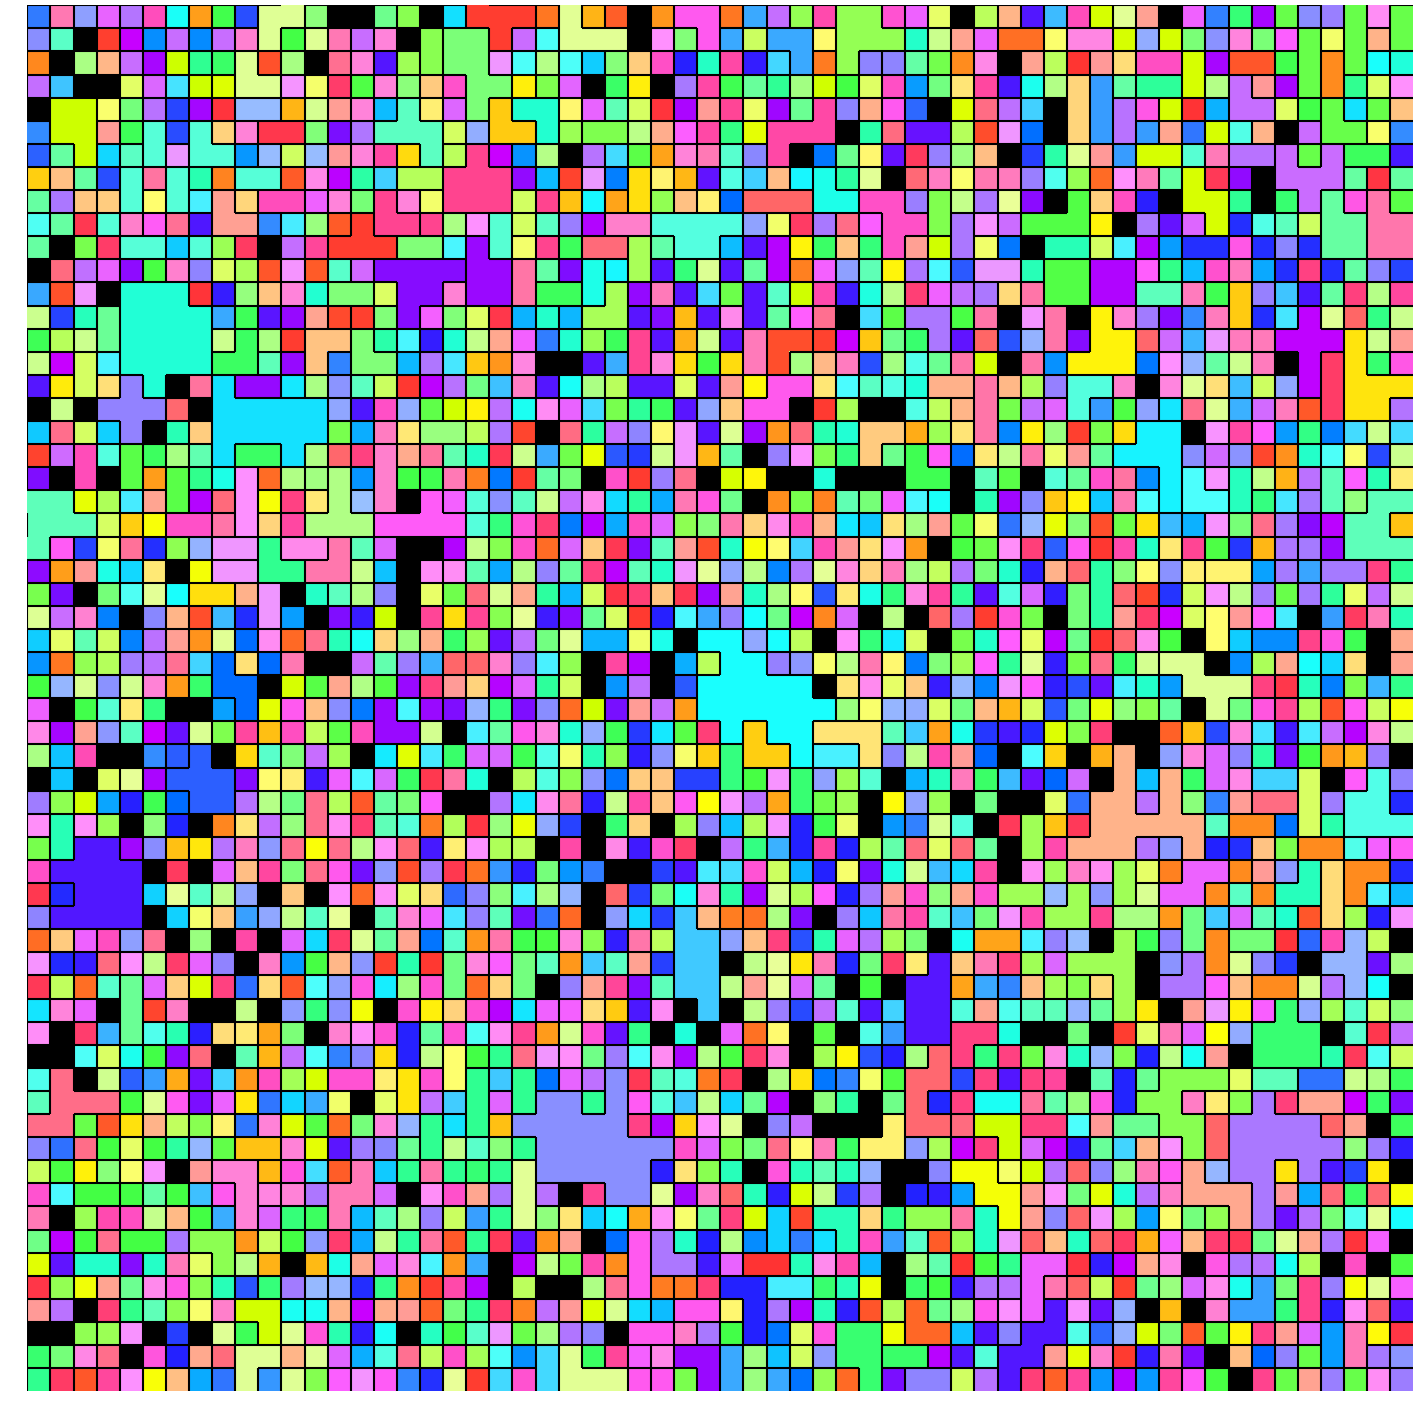
\includegraphics[width=\columnwidth]{seed=1001+title=channel_viz+treat=wave-big__mut-e_extreme+update=50000+_data_hathash_hash=6532b779898a7959+_script_fullcat_hash=474b4115ecde8750+_source_hash=d53f428-clean+ext=}
\end{subfigure}
\caption{
Representative same-channel signaling network end states for runs of each treatment.
A single cell-like organism occupies each grid tile except for black tiles, which are empty.
Channel IDs are coded by color.
Same-channel groups appear as uniformly-colored clumps, bounded by a black border.
}
\label{fig:outcome_grids}
\end{center}
\end{figure}


Indeed, in concordance with this second possibility, in Figure \ref{fig:outcome_grids} we can anecdotally observe more fragmented same-channel groups in treatments with greater mutational load.
This pattern is most strongly apparent in the large resource wave treatments, where the absence of large same-channel groups characteristic of low mutational load is easily observed under high mutational load, but also appears to hold for small resource wave treatments.
A more rigorous, quantitative analysis of this seeming pattern would benefit future work.

\begin{table}
 \centering
 \begin{tabular}{l c|cc} % alignment of each column data
 \multicolumn{4}{c}{\textbf{Extant Phylogenetic Roots}} \\
 & & \multicolumn{2}{c}{Resource Wave Size} \\
 & & Small & Large \\
 \hline
 \multirow{5}{*}{\STAB{\rotatebox[origin=c]{90}{\parbox{1.5cm}{\centering Mutational\\Load}}}} & 1 & $2 \pm 1$ & $61 \pm 52$ \\
 & 2 & $4 \pm 2$ & $80 \pm 51$\\
 & 3 & $5 \pm 1$ & $240 \pm 98$\\
 & 4 & $7 \pm 2$ & $599 \pm 82$\\
 & 5 & $28 \pm 3$ & $1204 \pm 116$\\
\end{tabular}
\caption{
Number of seed genomes with extant descendants (mean $\pm$ standard deviation across replicates).
}
\label{tab:phylogeny_roots}
\end{table}


The number of distinct phylogenetic roots among the extant population at the end of an evolutionary run provides a complimentary measure of evolutionary progress.
If only one phylogenetic root remains at the end of a run, the descendants of a single seeded cell have swept the entire population.
If two remain, the descendants of two distinct seeded cells are represented in the final population.
At the other end of the spectrum, 3600 phylogenetic roots would mean that a descendant from each and every seeded cell is present.
Table \ref{tab:phylogeny_roots} provides this metric for each treatment.
In agreement with Table \ref{tab:cell_generations}, the number of phylogenetic roots is lowest for low mutational load with small resource wave size (e.g., over more cellular generations, selection has eliminated a greater number of phylogenies) and the number of phylogenetic roots is greatest for high mutational load with large resource wave size (e.g., over fewer cellular generations, selection has yet to eliminate as many phylogenies).
From an evolutionary computing practitioner's perspective, the small number of extant phylogenies for low mutational load with small resource wave size --- generally, around two --- suggests that adaptive selection has strongly shaped the population in these replicates by the end of the evolutionary run.
However, the large number of extant phylogenies for high mutational load with large resource wave size --- generally, around 1200 --- suggests that adaptive selection has not as strongly shaped the population in these replicates by the end the of the evolutionary run.

With more computing time, we could extend the evolutionary runs of treatments with large resource wave size and/or larger mutational load in order to obtain populations with comparable evolutionary progress for all treatments.
However, we can still identify and discuss interesting differences between treatments while keeping this complicating factor in mind.

The central question we wish to answer:
